%% pernode.tex -- median wall-clock cost of one expansion, by algorithm and
%% connectivity (26-neighbour "diag" vs 6-neighbour "nodiag").
%% Generated fragment: wrap in \begin{figure}...\caption{...}\end{figure}.
%% Requires: tikz, pgfplots.
\begingroup
\pgfplotsset{compat=1.16}
\definecolor{pnDiag}{RGB}{20,66,110}
\definecolor{pnNodiagLine}{RGB}{176,74,16}
\definecolor{pnNodiagFill}{RGB}{247,203,167}
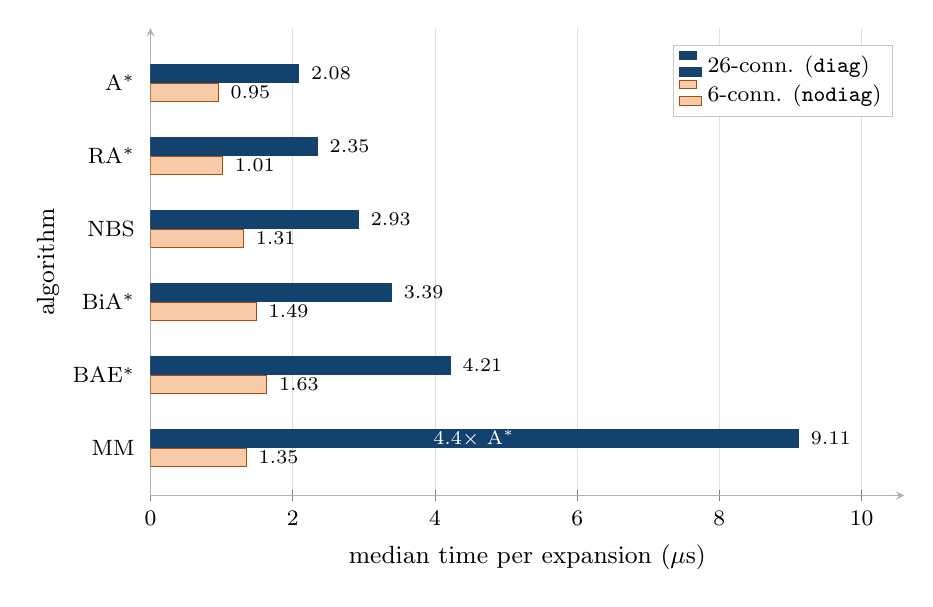
\begin{tikzpicture}
\begin{axis}[
  width=0.92\columnwidth, height=0.62\columnwidth,
  xbar,
  bar width=6.5pt,
  axis lines=left,
  axis line style={line width=0.35pt, draw=gray!60},
  xmin=0, xmax=10.6,
  ymin=0.35, ymax=6.75,
  enlargelimits=false,
  xtick={0,2,4,6,8,10},
  ytick={1,2,3,4,5,6},
  yticklabels={MM,BAE$^*$,BiA$^*$,NBS,RA$^*$,A$^*$},
  ytick style={draw=none},
  tick label style={font=\footnotesize},
  label style={font=\small},
  xlabel={median time per expansion ($\mu$s)},
  ylabel={algorithm},
  ylabel style={yshift=-2pt},
  xmajorgrids=true,
  grid style={line width=0.2pt, draw=gray!25},
  nodes near coords,
  point meta=x,
  every node near coord/.append style={font=\scriptsize, xshift=1pt,
      /pgf/number format/fixed, /pgf/number format/precision=2,
      /pgf/number format/fixed zerofill},
  legend style={font=\footnotesize, at={(0.985,0.965)}, anchor=north east,
                draw=gray!45, line width=0.3pt, fill=white, inner sep=2pt,
                row sep=-1pt},
  legend cell align=left,
]
%% 26-connected (diagonal moves allowed)
\addplot[bar shift=3.4pt, draw=pnDiag, line width=0.3pt, fill=pnDiag]
  coordinates {(2.0848,6) (2.3466,5) (2.9261,4) (3.3884,3) (4.2136,2) (9.1128,1)};
\addlegendentry{26-conn. (\texttt{diag})}
%% 6-connected (face moves only)
\addplot[bar shift=-3.4pt, draw=pnNodiagLine, line width=0.3pt, fill=pnNodiagFill]
  coordinates {(0.9525,6) (1.0139,5) (1.3076,4) (1.4879,3) (1.6335,2) (1.3471,1)};
\addlegendentry{6-conn. (\texttt{nodiag})}
%% MM's 26-connected outlier, relative to A* on the same graphs
\node[anchor=center, font=\scriptsize, text=white, yshift=3.4pt]
  at (axis cs:4.55,1) {$4.4\times$ A$^*$};
\end{axis}
\end{tikzpicture}
\endgroup
